% Shared preamble of the six stage reports (stages/README.md). Colours and notation are identical in every report.
\documentclass[11pt,a4paper]{article}
\usepackage[margin=2.2cm]{geometry}
\usepackage{amsmath,amssymb,booktabs,graphicx,xcolor,float,caption,subcaption,enumitem,longtable,array}
\usepackage[round]{natbib}
\usepackage[hidelinks]{hyperref}
\usepackage{fancyhdr}
\setlength{\emergencystretch}{2em}
\setlength{\parskip}{3pt}
\definecolor{roigreen}{RGB}{0,160,0}
\definecolor{artred}{RGB}{220,0,0}
\definecolor{maskblue}{RGB}{31,119,180}
\definecolor{ermgrey}{RGB}{110,110,110}
\definecolor{supported}{RGB}{0,120,0}
\definecolor{notsupported}{RGB}{190,0,0}
\newcommand{\ok}{\textcolor{supported}{\textbf{supported}}}
\newcommand{\no}{\textcolor{notsupported}{\textbf{not supported}}}
\newcommand{\mixed}{\textcolor{orange!80!black}{\textbf{partly supported}}}
\newcommand{\roi}{\textcolor{roigreen}{ROI}}
\newcommand{\na}{\textit{n/a}}
\newcommand{\registered}[1]{\textsf{registered before results (#1)}}
\newcommand{\posthoc}[1]{\textsf{post hoc (#1)}}
\pagestyle{fancy}\fancyhf{}\rhead{\small Where the Shortcut Sits --- stage reports}\lfoot{\small\leftmark}\rfoot{\small\thepage}
\newcommand{\stagebox}[1]{\noindent\colorbox{gray!12}{\parbox{\dimexpr\linewidth-2\fboxsep}{\small #1}}\par\medskip}

% generated by make_stage*.py from result files; do not edit
\providecommand{\sTwoMaskZero}{$+0.184$ [$+0.117, +0.250$]}
\providecommand{\sTwoMaskTwoFive}{$-0.059$ [$-0.127, +0.008$]}
\providecommand{\sTwoMaskFiveZero}{$-0.097$ [$-0.164, -0.030$]}
\providecommand{\sTwoMaskSevenFive}{$-0.111$ [$-0.181, -0.043$]}
\providecommand{\sTwoMaskOneZeroZero}{$-0.129$ [$-0.195, -0.064$]}
\providecommand{\sTwoInter}{$+0.313$ [$+0.258, +0.370$]}
\providecommand{\sTwoCorrMaskHundred}{0.961}
\providecommand{\sTwoCorrErmHundred}{0.937}
\providecommand{\sTwoCorrMaskZero}{0.849}
\providecommand{\sTwoRevMaskZero}{0.849}
\providecommand{\sTwoHarmVerdict}{lowers it significantly at 50, 75 and 100\% overlap}
\providecommand{\sTwoOccVerdict}{changes it significantly at none of the five overlaps (every CI includes zero)}
\providecommand{\sTwoDpMaskFull}{0.491}
\providecommand{\sTwoDpErmFull}{0.235}
\providecommand{\sTwoDpDiffFull}{$+0.255$ [$+0.221, +0.287$]}
\providecommand{\sTwoDpMaskZero}{0.000}
\providecommand{\sTwoDpErmZero}{0.128}
\providecommand{\sTwoSmallFull}{$-0.364$ [$-0.509, -0.217$]}
\providecommand{\sTwoLargeFull}{$+0.063$ [$-0.015, +0.144$]}
\providecommand{\sTwoLargeVerdict}{does not differ significantly from zero}
\providecommand{\sTwoDilFiveZeromZero}{$-0.097$ [$-0.164, -0.031$]}
\providecommand{\sTwoDilFiveZeromTwoFive}{$-0.153$ [$-0.221, -0.089$]}
\providecommand{\sTwoDilOneZeroZeromZero}{$-0.129$ [$-0.195, -0.066$]}
\providecommand{\sTwoDilOneZeroZeromFiveZero}{$-0.138$ [$-0.200, -0.082$]}
\providecommand{\sTwoRetFiveZeromZero}{0.500}
\providecommand{\sTwoShareFiveZeromZero}{0.028}
\providecommand{\sTwoRetFiveZeromTwoFive}{0.946}
\providecommand{\sTwoShareFiveZeromTwoFive}{0.026}
\providecommand{\sTwoRetOneZeroZeromZero}{0.999}
\providecommand{\sTwoShareOneZeroZeromZero}{0.055}
\providecommand{\sTwoRetOneZeroZeromFiveZero}{1.000}
\providecommand{\sTwoShareOneZeroZeromFiveZero}{0.018}
\providecommand{\sTwoDpRatioFull}{2.1}
\providecommand{\sTwoCfdermoscopyDINOvTwo}{$+0.255$ [$+0.221, +0.287$]}
\providecommand{\sTwoCfMaskdermoscopyDINOvTwo}{0.491}
\providecommand{\sTwoCfErmdermoscopyDINOvTwo}{0.235}
\providecommand{\sTwoCfthyroidDINOvTwo}{$+0.025$ [$-0.016, +0.065$]}
\providecommand{\sTwoCfMaskthyroidDINOvTwo}{0.393}
\providecommand{\sTwoCfErmthyroidDINOvTwo}{0.369}
\providecommand{\sTwoCfovaryDINOvTwo}{$+0.188$ [$+0.133, +0.250$]}
\providecommand{\sTwoCfMaskovaryDINOvTwo}{0.218}
\providecommand{\sTwoCfErmovaryDINOvTwo}{0.032}
\providecommand{\sTwoCfcapsuleDINOvTwo}{$+0.186$ [$+0.130, +0.260$]}
\providecommand{\sTwoCfMaskcapsuleDINOvTwo}{0.245}
\providecommand{\sTwoCfErmcapsuleDINOvTwo}{0.057}
\providecommand{\sTwoCfchestRADDINO}{$-0.127$ [$-0.136, -0.118$]}
\providecommand{\sTwoCfMaskchestRADDINO}{0.307}
\providecommand{\sTwoCfErmchestRADDINO}{0.434}
\providecommand{\sTwoCfNPos}{3}
\providecommand{\sTwoCfN}{5}
\providecommand{\sTwoTertLargeZero}{$+0.249$ [$+0.155, +0.346$]}
\providecommand{\sTwoTertLargeFiveZero}{$+0.087$ [$+0.006, +0.172$]}
\providecommand{\sTwoTertLargeOneZeroZero}{$+0.063$ [$-0.015, +0.144$]}
\providecommand{\sTwoRatioLarge}{0.012}
\providecommand{\sTwoTertMediumZero}{$+0.215$ [$+0.033, +0.391$]}
\providecommand{\sTwoTertMediumFiveZero}{$-0.129$ [$-0.283, +0.027$]}
\providecommand{\sTwoTertMediumOneZeroZero}{$-0.158$ [$-0.295, -0.027$]}
\providecommand{\sTwoRatioMedium}{0.031}
\providecommand{\sTwoTertSmallZero}{$+0.150$ [$+0.036, +0.273$]}
\providecommand{\sTwoTertSmallFiveZero}{$-0.326$ [$-0.471, -0.176$]}
\providecommand{\sTwoTertSmallOneZeroZero}{$-0.364$ [$-0.509, -0.217$]}
\providecommand{\sTwoRatioSmall}{0.106}
\providecommand{\sTwoCxrErmRevZero}{0.913}
\providecommand{\sTwoCxrMaskRevZero}{0.910}
\providecommand{\sTwoCxrErmRevOneZeroZero}{0.614}
\providecommand{\sTwoCxrMaskRevOneZeroZero}{0.725}
\providecommand{\sTwoCxrErmCleanZero}{0.915}
\providecommand{\sTwoCxrMaskCleanZero}{0.910}
\providecommand{\sTwoCxrErmCleanOneZeroZero}{0.907}
\providecommand{\sTwoCxrMaskCleanOneZeroZero}{0.904}
\providecommand{\sTwoCxrDinoErmRevZero}{0.629}
\providecommand{\sTwoCxrDinoMaskRevZero}{0.883}
\providecommand{\sTwoCxrDinoErmRevOneZeroZero}{0.410}
\providecommand{\sTwoCxrDinoMaskRevOneZeroZero}{0.327}
\providecommand{\sTwoCxrDinoErmCleanZero}{0.859}
\providecommand{\sTwoCxrDinoMaskCleanZero}{0.883}
\providecommand{\sTwoCxrDinoErmCleanOneZeroZero}{0.852}
\providecommand{\sTwoCxrDinoMaskCleanOneZeroZero}{0.867}
\providecommand{\sTwoThyroidcaliperDINOvTwoZero}{$+0.402$ [$+0.315, +0.489$]}
\providecommand{\sTwoThyroidcaliperDINOvTwoFull}{$-0.030$ [$-0.105, +0.042$]}
\providecommand{\sTwoThyroidcaliperDINOvTwoInter}{$+0.433$ [$+0.362, +0.507$]}
\providecommand{\sTwoThyroidcaliperMedSigLIPZero}{$+0.514$ [$+0.430, +0.600$]}
\providecommand{\sTwoThyroidcaliperMedSigLIPFull}{$+0.044$ [$-0.011, +0.104$]}
\providecommand{\sTwoThyroidcaliperMedSigLIPInter}{$+0.470$ [$+0.388, +0.556$]}
\providecommand{\sTwoOvariancaliperDINOvTwoZero}{$+0.041$ [$-0.096, +0.175$]}
\providecommand{\sTwoOvariancaliperDINOvTwoFull}{$-0.197$ [$-0.357, -0.035$]}
\providecommand{\sTwoOvariancaliperDINOvTwoInter}{$+0.238$ [$+0.144, +0.340$]}
\providecommand{\sTwoCapsuledebrisDINOvTwoZero}{$+0.116$ [$+0.052, +0.191$]}
\providecommand{\sTwoCapsuledebrisDINOvTwoFull}{$-0.112$ [$-0.209, -0.019$]}
\providecommand{\sTwoCapsuledebrisDINOvTwoInter}{$+0.228$ [$+0.144, +0.324$]}
\providecommand{\sTwoCapsuledebrisMedSigLIPZero}{$+0.374$ [$+0.248, +0.509$]}
\providecommand{\sTwoCapsuledebrisMedSigLIPFull}{$+0.216$ [$+0.118, +0.317$]}
\providecommand{\sTwoCapsuledebrisMedSigLIPInter}{$+0.158$ [$+0.012, +0.314$]}
\providecommand{\sTwoChesttubeRADDINOZero}{$-0.002$ [$-0.010, +0.005$]}
\providecommand{\sTwoChesttubeRADDINOFull}{$+0.111$ [$+0.095, +0.127$]}
\providecommand{\sTwoChesttubeRADDINOInter}{$-0.113$ [$-0.129, -0.097$]}
\providecommand{\sTwoChesttubeDINOvTwoZero}{$+0.254$ [$+0.230, +0.278$]}
\providecommand{\sTwoChesttubeDINOvTwoFull}{$-0.083$ [$-0.112, -0.057$]}
\providecommand{\sTwoChesttubeDINOvTwoInter}{$+0.337$ [$+0.312, +0.364$]}
\providecommand{\sTwoDinoTwoTwoFourInter}{$+0.456$ [$+0.390, +0.525$]}
\providecommand{\sTwoDermlipInter}{$+0.424$ [$+0.335, +0.517$]}
\providecommand{\sTwoStressInter}{$+0.302$ [$+0.248, +0.357$]}
\providecommand{\sTwoNSweeps}{11}
\providecommand{\sTwoNInterPos}{10}
\providecommand{\sTwoNInterNeg}{1}
\providecommand{\sTwoNHarmFull}{7}
\providecommand{\sTwoNHelpFull}{2}
\providecommand{\sTwoNNullFull}{2}
\providecommand{\sTwoRegRep}{\texttt{2699d51}, 2026-09-26 15:47}
\providecommand{\sTwoRegFinal}{\texttt{c45d482}, 2026-09-28 00:35}
\providecommand{\sTwoRegThy}{\texttt{ea57661}, 2026-09-26 22:46}
\providecommand{\sTwoRegOv}{\texttt{2517600}, 2026-09-27 07:29}
\providecommand{\sTwoRegCap}{\texttt{fcbf8d9}, 2026-09-27 00:40}
\providecommand{\sTwoRegCxr}{\texttt{4d1a924}, 2026-09-26 18:07}
\providecommand{\sTwoRegRev}{\texttt{29cd0da}, 2026-09-27 18:56}
\providecommand{\sTwoThyroidcaliperDINOvTwoBalInter}{$-0.076$ [$-0.106, -0.048$]}
\providecommand{\sTwoThyroidcaliperMedSigLIPBalInter}{$-0.052$ [$-0.084, -0.020$]}
\providecommand{\sTwoOvariancaliperDINOvTwoBalInter}{$-0.018$ [$-0.048, +0.009$]}
\providecommand{\sTwoCapsuledebrisDINOvTwoBalInter}{$-0.032$ [$-0.073, +0.001$]}
\providecommand{\sTwoCapsuledebrisMedSigLIPBalInter}{$-0.245$ [$-0.359, -0.130$]}
\providecommand{\sTwoChesttubeRADDINOBalInter}{$-0.309$ [$-0.338, -0.281$]}
\providecommand{\sTwoChesttubeDINOvTwoBalInter}{$-0.214$ [$-0.231, -0.196$]}
\providecommand{\sTwoDermBalInter}{$-0.143$ [$-0.171, -0.119$]}
\providecommand{\sTwoDermInpInter}{$-0.103$ [$-0.127, -0.080$]}
\providecommand{\sTwoEstN}{180}
\providecommand{\sTwoEstLost}{11}
\providecommand{\sTwoEstGained}{0}
\providecommand{\sTwoEstMed}{1.45}

\newcommand{\notY}{1 = melanoma (dermoscopy), malignant nodule (thyroid), tumour with a solid component (ovary), erosion (capsule), pneumothorax (chest radiograph)}
\newcommand{\notA}{a synthetic artifact pasted at a controlled position: ruler (dermoscopy), sonographer caliper (thyroid, ovary), debris blob (capsule endoscopy), tube (chest radiograph)}
\newcommand{\notROI}{lesion, nodule, tumour, annotated lesion box, lungs}
\newcommand{\notCross}{the \emph{location interaction} $[\text{mask}-\text{ERM}]_{r=0}-[\text{mask}-\text{ERM}]_{r=1}$ of reversed-test AUROC on the same images.}
\newcommand{\notCI}{95\% crossed seed$\times$image bootstrap interval (Stage~1); every interval in this report uses it.}
\newcommand{\notExtra}{}
\title{\textbf{Stage 2 --- The location law and its mechanism}\\[3pt]\large Where the Shortcut Sits: progress report 2}
\author{}
\date{}
\begin{document}
\maketitle
\stagebox{\textbf{In one sentence.} When only the artifact's overlap with the region of interest (ROI) is varied,
ROI masking helps while the artifact lies outside the ROI and loses its benefit --- in 7 of 11 sweeps it hurts ---
once the artifact overlaps it; the reversal comes from the artifact \emph{surviving} the mask and becoming what the model
relies on, not from occlusion; and it recurs in thyroid and ovarian ultrasound, capsule endoscopy and chest
radiography, with one principled exception (an encoder that ignores an artifact outside the lungs).}
% Shared notation. Each stage defines \notY, \notA, \notROI, \notCross, \notCI and \notExtra before \input-ing this
% file, so that a report only names the cohorts and quantities it has already introduced.
\section*{Notation}
\begin{tabular}{p{3.2cm}p{11.8cm}}
$Y\in\{0,1\}$ & diagnosis: \notY. \\
$A\in\{0,1\}$ & artifact present: \notA. \\
ROI & region of interest: \notROI; drawn in \textcolor{roigreen}{green}; artifacts in \textcolor{artred}{red}. \\
$r$ & overlap $|\text{artifact}\cap\text{ROI}|/|\text{artifact}|$. Trap~A: $r\ge0.5$ (artifact in the ROI); Trap~B: $r<0.1$ (outside). \\
Environments & training and correlated test $P(A{=}1\mid Y{=}1)=0.9$, $P(A{=}1\mid Y{=}0)=0.1$; reversed test 0.1/0.9; clean test: artifact independent of $Y$ (real artifacts: half of each class) or absent (synthetic artifacts). \\
ERM, mask & linear head on the frozen features of the original image / of the ROI-masked image. \\
Crossover & \notCross \\
CI & \notCI \\
$|\Delta p|$ & same-head counterfactual sensitivity: change of the predicted probability when the artifact is inserted into the same image. \\
\notExtra
\end{tabular}


\tableofcontents
\clearpage

\section{Where this stage starts}
Stage~1 re-derived the pilot and fixed the protocol: trap environments, frozen foundation-model features, linear heads
chosen on clean validation data, grouped splits, pre-registration and the crossed bootstrap. It showed that the
pilot's central observation replicates: in the controlled dermoscopy sweep, masking changes reversed-test AUROC from
\sTwoMaskZero{} at 0\% overlap to \sTwoMaskOneZeroZero{} at 100\% overlap. Stage~1 deliberately did not interpret the
pilot's mechanism experiments. This stage asks the two questions that follow: \emph{why} does masking reverse, and
\emph{how general} is the reversal --- does it depend on dermoscopy, on the ruler, on DINOv2?

\section{Questions}
\begin{enumerate}[label=\textbf{Q2\alph*},leftmargin=*]\itemsep1pt
\item Is the benefit of masking a function of the artifact's overlap $r$ with the ROI, falling from $r=0$ to $r=1$?
We call a positive location interaction $\big[\mathrm{mask}-\mathrm{ERM}\big]_{r=0}-\big[\mathrm{mask}-\mathrm{ERM}\big]_{r=1}$
on the reversed test the \emph{location law}.
\item Which mechanism produces the fall? Three candidates were stated in advance: \emph{occlusion} (masking removes
useful context whatever the artifact does), \emph{lost disease signal} (the background carries diagnostic
information), and \emph{retention with amplified reliance} (the part of the artifact inside the ROI survives masking,
its competitors are removed, and the head relies on it more).
\item Does the law hold beyond one encoder, one artifact rendering and one modality --- and where does it fail?
\end{enumerate}

\subsection{Why these experiments, and what was rejected}
\begin{itemize}[leftmargin=*]\itemsep1pt
\item \emph{An occlusion control instead of an argument from intuition.} If masking harmed because it throws away
context, it would harm even when the artifact carries no label information \citep[cf.][]{fong2019occlusions}. The
control keeps the ruler at the same positions but makes it independent of the label.
\item \emph{Dilation as a dose of retention.} Growing the mask by a margin keeps more of the ruler visible without
changing the lesion. If retention drives the harm, harm should grow with retention when retention is incomplete (50\%
overlap) and stay flat when the ruler is already fully retained (100\% overlap) --- even though dilation then
\emph{lowers} the ruler's share of the visible pixels.
\item \emph{A same-head counterfactual instead of saliency maps.} Saliency maps are qualitative and unstable for frozen
encoders. Instead, the ruler is inserted into and removed from the \emph{same} test image and the change in each
trained head's predicted probability, $|\Delta p|$, is read: a direct, per-image measure of reliance on the artifact.
\item \emph{Lesion size as a natural dose.} The same ruler covers a larger share of a small lesion. If what matters is
how dominant the retained artifact is among the remaining evidence, harm should be largest for small lesions. No
threshold ratio was pre-specified, because the pilot showed none.
\item \emph{Other modalities with their own artifact.} A caliper drawn like a sonographer's, a debris blob drawn like
capsule contamination and a tube drawn like a drain, each pasted at controlled overlap on real images of that modality
with that modality's own ROI masks. This tests whether the law is a property of dermoscopy or of masking.
\item \emph{Rejected:} measuring reliance through head weights (they are not comparable between masked and unmasked
feature spaces), and a single ``average'' overlap (it would hide the sign change).
\end{itemize}

\section{Methods}
\paragraph{Controlled dermoscopy sweep} As in Stage~1: ISIC 2018 pilot cohort, a $65\times19$\,px ruler at a frozen
position per image and overlap $r\in\{0,0.25,0.5,0.75,1\}$; DINOv2 ViT-B/14 at 518\,px \citep{oquab2024dinov2} (CLS
features), logistic heads, seeds 42, 123, 456; primary outcome reversed-test AUROC.
\paragraph{Arms} ERM; ROI masking; oracle inpainting of the ruler; group-balanced reweighting; DFR
\citep{kirichenko2023dfr}; paired LEACE \citep{belrose2023leace}; GroupDRO \citep{sagawa2020groupdro}. All arms share
features and seeds; only the input or the head changes.
\paragraph{Occlusion control} The ruler is pasted at the same positions in 50\% of images independently of the label;
AUROC is measured on a 50/50 test.
\paragraph{Mask dilation} The lesion mask is dilated by 0, 10, 25 or 50\,px before masking. \emph{Retention} is the share
of ruler pixels that remain visible; \emph{ruler share} is the ruler's share of all visible pixels.
\paragraph{Same-head counterfactual} For each artifact-bearing image of the reversed test and each trained head, the
image is scored with and without the pasted artifact (the masked head sees the masked version of both); $|\Delta p|$ is
the absolute change in predicted probability. The mask $-$ ERM difference of mean $|\Delta p|$ is bootstrapped with
seeds and images crossed.
\paragraph{Lesion-size strata} Test images are split into tertiles of lesion area; the median ruler-to-lesion area
ratio is reported per tertile.
\paragraph{Replications} DINOv2 at 224\,px, DermLIP at 224\,px \citep{yan2025derm1m}, and a ruler whose colour, tick
pattern and size are randomised per image (``stress'').
\paragraph{Other modalities} Each sweep uses only images of that cohort in which the real artifact is absent, so that
the pasted artifact is the only one:
\begin{itemize}[leftmargin=*]\itemsep1pt
\item \textbf{Thyroid ultrasound} (TN3K images with TNCD malignancy labels and manual nodule masks \citep{gong2021tn3k};
1,663 caliper-free images): a synthetic sonographer caliper (dotted line with ``+'' ends) in the same $65\times19$ box
as the ruler; DINOv2 and MedSigLIP-448. Split: official TN3K test images as test; the rest 80/20 by leakage group.
\item \textbf{Ovarian ultrasound} (MMOTU OTU\_2d \citep{zhao2022mmotu}; benign cystic lesions versus tumours with a
solid component; 343 caliper-free images, 64 in test): the same caliper; DINOv2. Small, so wide intervals were
expected.
\item \textbf{Capsule endoscopy} (SEE-AI \citep{seeai2023}; erosion versus polyp-like lesions; ROI = the union of the
expert lesion boxes; 796 low-contamination frames, split 60/20/20 by frame-block group): a textured yellow-green debris
blob with bubbles, $48\times48$\,px; DINOv2 and MedSigLIP.
\item \textbf{Chest radiography} (NIH ChestX-ray14 pneumothorax \citep{wang2017chestxray8}; lung masks from a PSPNet
\citep{cohen2022xrv}; patient-grouped split): a synthetic tube; RAD-DINO @518 \citep{perezgarcia2025raddino} (a
chest-radiograph foundation model) and DINOv2.
\end{itemize}
Figure~\ref{fig:examples} shows three of these sweeps on real images.
\paragraph{Statistics} Every interval is a 95\% percentile interval from 10,000 crossed bootstrap replicates.
``Significant'' means the 95\% interval excludes zero; it is not a multiplicity-adjusted test.

\section{Experiments}
Table~\ref{tab:exp} lists each experiment of this stage with its registration and support criterion. The dermoscopy
analyses (E1--E7) were specified in the pilot specification (\sTwoRegRep); the other-modality sweeps were registered
with their cohorts before any model was fitted. The DINOv2 chest-tube sweep was added after the RAD-DINO result and is
labelled post hoc.
\begin{table}[H]\centering\scriptsize
\caption{Experiments of this stage: registration status, the registration document (\texttt{docs/PREREGISTRATION\_<name>.md} or the replication specification), the commit that first contains it, and what was stated in advance to count as support. Commit times are set by the committing machine and are not independent proof of order.}\label{tab:exp}
\begin{tabular}{p{3.1cm}p{2.1cm}p{2.4cm}p{3.2cm}p{3.3cm}}\toprule
Experiment & Status & Registration & First commit (local time) & Support criterion \\\midrule
Controlled dermoscopy sweep (E1) & \ok{} registered & REPLICATION\_\allowbreak{}SPEC & \texttt{2699d51}, 2026-09-26 15:47 & interaction CI $>0$; mask$-$ERM CI $>0$ at 0\% and $<0$ at 100\% \\
Replications: DINOv2@224, DermLIP, randomised ruler & \ok{} registered & REPLICATION\_\allowbreak{}SPEC & \texttt{2699d51}, 2026-09-26 15:47 & same signs and verdicts as E1 \\
Occlusion control (E4) & \ok{} registered & REPLICATION\_\allowbreak{}SPEC & \texttt{2699d51}, 2026-09-26 15:47 & no harm on the 50/50 test at any overlap \\
Mask dilation (E5) & \ok{} registered & REPLICATION\_\allowbreak{}SPEC & \texttt{2699d51}, 2026-09-26 15:47 & harm grows with retention at 50\%; flat at 100\% \\
Same-head counterfactual $|\Delta p|$ (E6, T3) & \ok{} registered & REVIEW2 (T3) & \texttt{29cd0da}, 2026-09-27 18:56 & mask $>$ ERM at in-ROI overlap, CI $>0$ \\
Lesion-size tertiles (E7) & \mixed{} pilot analysis, replicated & REPLICATION\_\allowbreak{}SPEC & \texttt{2699d51}, 2026-09-26 15:47 & harm largest in small lesions \\
Thyroid caliper sweep & \ok{} registered & THYROID\_\allowbreak{}TRAPS & \texttt{ea57661}, 2026-09-26 22:46 & interaction CI $>0$ \\
Ovarian caliper sweep & \ok{} registered & OVARY\_\allowbreak{}TRAPS & \texttt{2517600}, 2026-09-27 07:29 & interaction CI $>0$ \\
Capsule debris sweep & \ok{} registered & CAPSULE\_\allowbreak{}TRAPS & \texttt{fcbf8d9}, 2026-09-27 00:40 & interaction CI $>0$ \\
Chest tube sweep (RAD-DINO) & \ok{} registered & CXR\_\allowbreak{}DEVICE\_\allowbreak{}TRAPS & \texttt{4d1a924}, 2026-09-26 18:07 & interaction CI $>0$ \\
Chest tube sweep (DINOv2) & \no{} post hoc & --- & --- & descriptive only \\
Crossed-bootstrap intervals for every sweep (A1) & \ok{} registered & FINAL (A1) & \texttt{c45d482}, 2026-09-28 00:35 & a claim is stated only if its crossed CI excludes 0 \\
\bottomrule\end{tabular}
\end{table}


\section{Results}
\subsection{The dermoscopy sweep: every arm, every overlap}
Masking changes the reversed-test AUROC by \sTwoMaskZero{} when the ruler lies outside the lesion, by
\sTwoMaskFiveZero{} at 50\% overlap and by \sTwoMaskOneZeroZero{} at full overlap (Table~\ref{tab:sweep}); the location
interaction is \sTwoInter. Masking therefore \sTwoHarmVerdict. Every other arm helps at every overlap, and their
benefit \emph{grows} with overlap --- the opposite of masking: balancing's location interaction is \sTwoDermBalInter,
inpainting's \sTwoDermInpInter. They target the artifact, not the background, and the ERM shortcut they remove is
larger when the ruler sits on the lesion. On the correlated test the masked model at full overlap scores
\sTwoCorrMaskHundred{} against \sTwoCorrErmHundred{} for ERM: the masked model exploits the ruler more.
\begin{table}[H]\centering\small
\caption{Controlled dermoscopy sweep (ISIC 2018, DINOv2 ViT-B/14 @518, three seeds): change in reversed-test AUROC versus ERM, crossed CIs.}\label{tab:sweep}
\resizebox{\linewidth}{!}{\begin{tabular}{lccc}\toprule
 & 0\% overlap & 50\% & 100\% \\\midrule
ERM (reversed AUROC) & 0.665 & 0.573 & 0.515 \\
ROI masking $-$ ERM & $+0.184$ [$+0.117, +0.250$] & $-0.097$ [$-0.164, -0.030$] & $-0.129$ [$-0.195, -0.064$] \\
oracle inpainting $-$ ERM & $+0.141$ [$+0.109, +0.175$] & $+0.211$ [$+0.175, +0.249$] & $+0.243$ [$+0.205, +0.284$] \\
group-balanced $-$ ERM & $+0.137$ [$+0.099, +0.179$] & $+0.219$ [$+0.177, +0.265$] & $+0.281$ [$+0.236, +0.329$] \\
DFR $-$ ERM & $+0.124$ [$+0.075, +0.179$] & $+0.221$ [$+0.166, +0.281$] & $+0.279$ [$+0.220, +0.339$] \\
paired LEACE $-$ ERM & $+0.167$ [$+0.126, +0.211$] & $+0.237$ [$+0.197, +0.280$] & $+0.294$ [$+0.249, +0.339$] \\
GroupDRO $-$ ERM & $+0.080$ [$+0.044, +0.118$] & $+0.152$ [$+0.112, +0.193$] & $+0.197$ [$+0.155, +0.240$] \\
\bottomrule\end{tabular}}
\end{table}

\paragraph{Replications} The sweep reverses with DINOv2 at 224\,px (interaction \sTwoDinoTwoTwoFourInter), with DermLIP
(\sTwoDermlipInter) and with a randomised ruler (\sTwoStressInter) (Table~\ref{tab:rep}).
\begin{table}[H]\centering\small
\caption{Replications of the controlled sweep (reversed-test AUROC, crossed CIs).}\label{tab:rep}
\resizebox{\linewidth}{!}{\begin{tabular}{lccc}\toprule
Backbone / artifact & mask $-$ ERM at 0\% & at 100\% & Location interaction \\\midrule
DINOv2 @224 & $+0.361$ [$+0.275, +0.444$] & $-0.095$ [$-0.156, -0.035$] & $+0.456$ [$+0.390, +0.525$] \\
DermLIP @224 & $+0.161$ [$+0.102, +0.222$] & $-0.263$ [$-0.348, -0.180$] & $+0.424$ [$+0.335, +0.517$] \\
DINOv2 @518, randomised ruler & $+0.146$ [$+0.082, +0.211$] & $-0.155$ [$-0.228, -0.084$] & $+0.302$ [$+0.248, +0.357$] \\
\bottomrule\end{tabular}}
\end{table}


\subsection{Mechanism}
\paragraph{Occlusion does not explain the harm} With the ruler present but uninformative, masking \sTwoOccVerdict{}
(Table~\ref{tab:occ}); inpainting, which removes only the ruler, changes nothing either. Masking by itself does not cost
the reversed-test AUROC it loses in the sweep.
\begin{table}[H]\centering\small
\caption{Occlusion control: ruler present but uncorrelated with the label (50/50); AUROC change on the 50/50 test.}\label{tab:occ}
\begin{tabular}{lcc}\toprule
Overlap & mask $-$ ERM & inpaint $-$ ERM \\\midrule
0\% & $+0.036$ [$-0.016, +0.086$] & $-0.001$ [$-0.005, +0.003$] \\
25\% & $+0.022$ [$-0.030, +0.073$] & $-0.010$ [$-0.034, +0.002$] \\
50\% & $+0.041$ [$-0.010, +0.090$] & $-0.002$ [$-0.007, +0.003$] \\
75\% & $+0.037$ [$-0.013, +0.086$] & $-0.003$ [$-0.008, +0.001$] \\
100\% & $+0.039$ [$-0.010, +0.091$] & $-0.004$ [$-0.010, +0.002$] \\
\bottomrule\end{tabular}
\end{table}


\paragraph{Harm follows the visibility of the artifact} At 50\% overlap, dilating the mask from 0 to 25\,px raises
retention from \sTwoRetFiveZeromZero{} to \sTwoRetFiveZeromTwoFive{} and moves the masking effect from
\sTwoDilFiveZeromZero{} to \sTwoDilFiveZeromTwoFive. At 100\% overlap the ruler is already retained
(\sTwoRetOneZeroZeromZero) and the effect stays flat (\sTwoDilOneZeroZeromZero{} without and \sTwoDilOneZeroZeromFiveZero{}
with a 50\,px margin), although dilation \emph{lowers} the ruler's share of the visible pixels threefold
(\sTwoShareOneZeroZeromZero{} to \sTwoShareOneZeroZeromFiveZero). Harm therefore tracks whether the ruler is visible, not
how much of the image it occupies once visible (Table~\ref{tab:dil}). This also rules out ``lost context'' as the sole
cause: dilation \emph{restores} context, yet harm grows at 50\% overlap. The intervals of neighbouring margins overlap;
the pattern, not each step, is the finding.
\begin{table}[H]\centering\small
\caption{Mask dilation: restoring context around the lesion restores ruler pixels (retention) and changes harm.}\label{tab:dil}
\begin{tabular}{lcccc}\toprule
Overlap & Margin (px) & Ruler retained & Ruler share of visible pixels & mask $-$ ERM (rev) \\\midrule
50\% & 0 & 0.500 & 0.028 & $-0.097$ [$-0.164, -0.031$] \\
 & 10 & 0.725 & 0.029 & $-0.138$ [$-0.203, -0.074$] \\
 & 25 & 0.946 & 0.026 & $-0.153$ [$-0.221, -0.089$] \\
 & 50 & 1.000 & 0.018 & $-0.142$ [$-0.206, -0.083$] \\
75\% & 0 & 0.750 & 0.042 & $-0.111$ [$-0.181, -0.044$] \\
 & 10 & 0.940 & 0.037 & $-0.152$ [$-0.217, -0.091$] \\
 & 25 & 1.000 & 0.028 & $-0.160$ [$-0.226, -0.096$] \\
 & 50 & 1.000 & 0.018 & $-0.140$ [$-0.201, -0.079$] \\
100\% & 0 & 0.999 & 0.055 & $-0.129$ [$-0.195, -0.066$] \\
 & 10 & 1.000 & 0.040 & $-0.144$ [$-0.206, -0.082$] \\
 & 25 & 1.000 & 0.028 & $-0.144$ [$-0.209, -0.082$] \\
 & 50 & 1.000 & 0.018 & $-0.138$ [$-0.200, -0.082$] \\
\bottomrule\end{tabular}
\end{table}


\paragraph{The masked model relies more on the retained artifact} On the same images, inserting the ruler at full
overlap changes the masked head's prediction by \sTwoDpMaskFull{} on average and the ERM head's by \sTwoDpErmFull{}
--- about \sTwoDpRatioFull{} times as much; the paired difference is \sTwoDpDiffFull{} (Table~\ref{tab:cf},
Figure~\ref{fig:cf}). At 0\% overlap the masked head cannot see the ruler (\sTwoDpMaskZero) whereas ERM still reacts to it
(\sTwoDpErmZero). This is the mechanism in one measurement: masking removes the competing evidence, the retained
artifact becomes the most informative remaining feature, and the head leans on it. Across the \sTwoCfN{} sweeps with
counterfactual scores the masked head is significantly more sensitive at full overlap in \sTwoCfNPos: ovarian calipers
(\sTwoCfMaskovaryDINOvTwo{} versus \sTwoCfErmovaryDINOvTwo; \sTwoCfovaryDINOvTwo) and capsule debris
(\sTwoCfMaskcapsuleDINOvTwo{} versus \sTwoCfErmcapsuleDINOvTwo; \sTwoCfcapsuleDINOvTwo) besides the ruler. For thyroid
calipers the two heads are equally sensitive (\sTwoCfthyroidDINOvTwo) --- ERM already relies heavily on a caliper inside
the nodule --- and with RAD-DINO the masked head is \emph{less} sensitive to an in-lung tube (\sTwoCfchestRADDINO).
\begin{table}[H]\centering\scriptsize
\caption{Same-head counterfactual sensitivity to inserting the artifact (reversed test, artifact-bearing images), crossed CIs of the paired difference.}\label{tab:cf}
\resizebox{\linewidth}{!}{\begin{tabular}{lcccc}\toprule
Sweep & Overlap & $|\Delta p|$ ERM & $|\Delta p|$ mask & mask $-$ ERM \\\midrule
dermoscopy ruler (DINOv2) & 0\% & 0.128 & 0.000 & $-0.128$ [$-0.136, -0.121$] \\
 & 25\% & 0.190 & 0.353 & $+0.162$ [$+0.136, +0.188$] \\
 & 50\% & 0.195 & 0.399 & $+0.204$ [$+0.177, +0.230$] \\
 & 75\% & 0.197 & 0.422 & $+0.225$ [$+0.195, +0.255$] \\
 & 100\% & 0.235 & 0.491 & $+0.255$ [$+0.221, +0.287$] \\
\bottomrule\end{tabular}}
\end{table}

\begin{figure}[H]\centering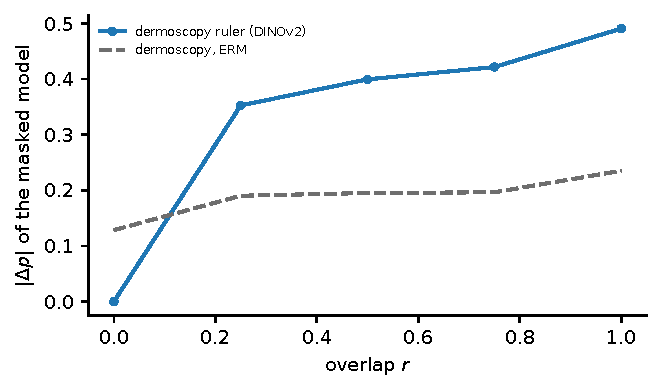
\includegraphics[width=0.66\linewidth]{figures/counterfactual.pdf}
\caption{Mean same-head sensitivity $|\Delta p|$ to inserting the artifact: masked model per sweep (solid) and ERM
for the dermoscopy sweep (dashed), by overlap.}\label{fig:cf}\end{figure}

\paragraph{Lesion size} Table~\ref{tab:tert}. The ruler covers a median \sTwoRatioLarge{} of a large lesion's area,
\sTwoRatioMedium{} of a medium and \sTwoRatioSmall{} of a small one. The harm at full overlap is significant for small
(\sTwoTertSmallOneZeroZero) and medium lesions (\sTwoTertMediumOneZeroZero) and not for large ones
(\sTwoTertLargeOneZeroZero, which \sTwoLargeVerdict); at 50\% overlap it is significant only for small lesions
(\sTwoTertSmallFiveZero; medium \sTwoTertMediumFiveZero). What holds is an ordering --- harm is largest where the
artifact is large relative to the lesion --- with wide intervals, because each tertile has few melanomas. No fixed ratio
threshold is claimed.
\begin{table}[H]\centering\scriptsize
\caption{Lesion-size strata of the controlled sweep (reversed-test AUROC, crossed CIs).}\label{tab:tert}
\resizebox{\linewidth}{!}{\begin{tabular}{lccccc}\toprule
Lesion tertile & Ruler/lesion area (median) & Melanomas in test & mask $-$ ERM at 0\% & 50\% & 100\% \\\midrule
large & 0.012 & 36 & $+0.249$ [$+0.155, +0.346$] & $+0.087$ [$+0.006, +0.172$] & $+0.063$ [$-0.015, +0.144$] \\
medium & 0.031 & 21 & $+0.215$ [$+0.033, +0.391$] & $-0.129$ [$-0.283, +0.027$] & $-0.158$ [$-0.295, -0.027$] \\
small & 0.106 & 16 & $+0.150$ [$+0.036, +0.273$] & $-0.326$ [$-0.471, -0.176$] & $-0.364$ [$-0.509, -0.217$] \\
\bottomrule\end{tabular}}
\end{table}


\paragraph{Synthesis} Occlusion alone does not harm; restoring context does not remove the harm; harm follows whether
the artifact is visible after masking, and the masked model's reliance on a visible artifact is larger than ERM's.
The mechanism is \emph{retention with amplified reliance}: masking deletes the out-of-ROI evidence --- including other
cues that competed with the artifact --- and leaves the in-ROI artifact as a larger share of what predicts the label in
training, so the head weights it more heavily.

\subsection{Other modalities}
\begin{figure}[H]\centering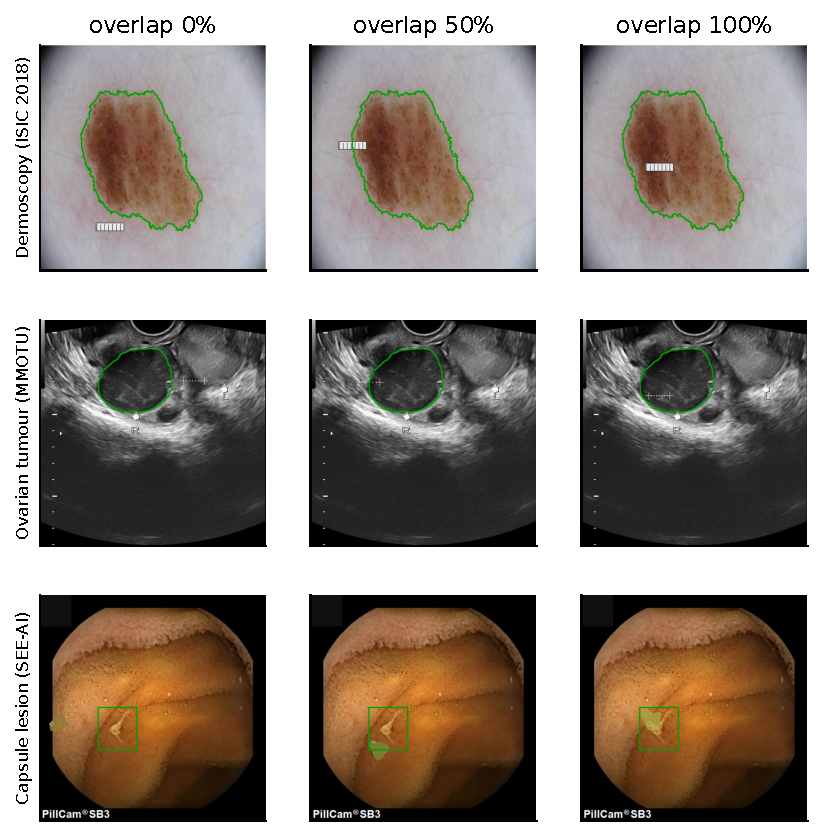
\includegraphics[width=0.86\linewidth]{figures/sweep_examples.pdf}
\caption{Real images with the synthetic artifact at 0, 50 and 100\% overlap (\textcolor{roigreen}{green}: ROI; the
capsule ROI is the annotated bounding box). Top: ISIC 2018 (CC BY-NC 4.0); middle: MMOTU ovarian ultrasound (CC BY
4.0); bottom: SEE-AI capsule endoscopy (CC BY 4.0). Thyroid (TN3K) and NIH images are not shown because their
redistribution terms are unclear.}\label{fig:examples}\end{figure}
Table~\ref{tab:other} and Figure~\ref{fig:doseall} repeat the sweep in four further modalities; Table~\ref{tab:otherarms}
gives every baseline arm. Across all \sTwoNSweeps{} controlled sweeps (four dermoscopy, seven others) the location
interaction is positive with an interval above zero in \sTwoNInterPos{} and negative in \sTwoNInterNeg. Whether the
falling benefit turns into harm at full overlap depends on the setting: masking harms significantly at full overlap in
\sTwoNHarmFull{} sweeps, still helps in \sTwoNHelpFull{} and makes no significant difference in \sTwoNNullFull.
\begin{table}[H]\centering\scriptsize
\caption{Controlled sweeps in the other modalities (synthetic caliper, debris, tube pasted at controlled overlap; reversed-test AUROC, crossed CIs).}\label{tab:other}
\resizebox{\linewidth}{!}{\begin{tabular}{lccc}\toprule
Sweep & mask $-$ ERM at 0\% & at 100\% & Location interaction \\\midrule
Thyroid caliper, DINOv2 & $+0.402$ [$+0.315, +0.489$] & $-0.030$ [$-0.105, +0.042$] & $+0.433$ [$+0.362, +0.507$] \\
Thyroid caliper, MedSigLIP & $+0.514$ [$+0.430, +0.600$] & $+0.044$ [$-0.011, +0.104$] & $+0.470$ [$+0.388, +0.556$] \\
Ovarian caliper, DINOv2 & $+0.041$ [$-0.096, +0.175$] & $-0.197$ [$-0.357, -0.035$] & $+0.238$ [$+0.144, +0.340$] \\
Capsule debris, DINOv2 & $+0.116$ [$+0.052, +0.191$] & $-0.112$ [$-0.209, -0.019$] & $+0.228$ [$+0.144, +0.324$] \\
Capsule debris, MedSigLIP & $+0.374$ [$+0.248, +0.509$] & $+0.216$ [$+0.118, +0.317$] & $+0.158$ [$+0.012, +0.314$] \\
Chest tube, RAD-DINO & $-0.002$ [$-0.010, +0.005$] & $+0.111$ [$+0.095, +0.127$] & $-0.113$ [$-0.129, -0.097$] \\
Chest tube, DINOv2 & $+0.254$ [$+0.230, +0.278$] & $-0.083$ [$-0.112, -0.057$] & $+0.337$ [$+0.312, +0.364$] \\
\bottomrule\end{tabular}}
\end{table}

\begin{figure}[H]\centering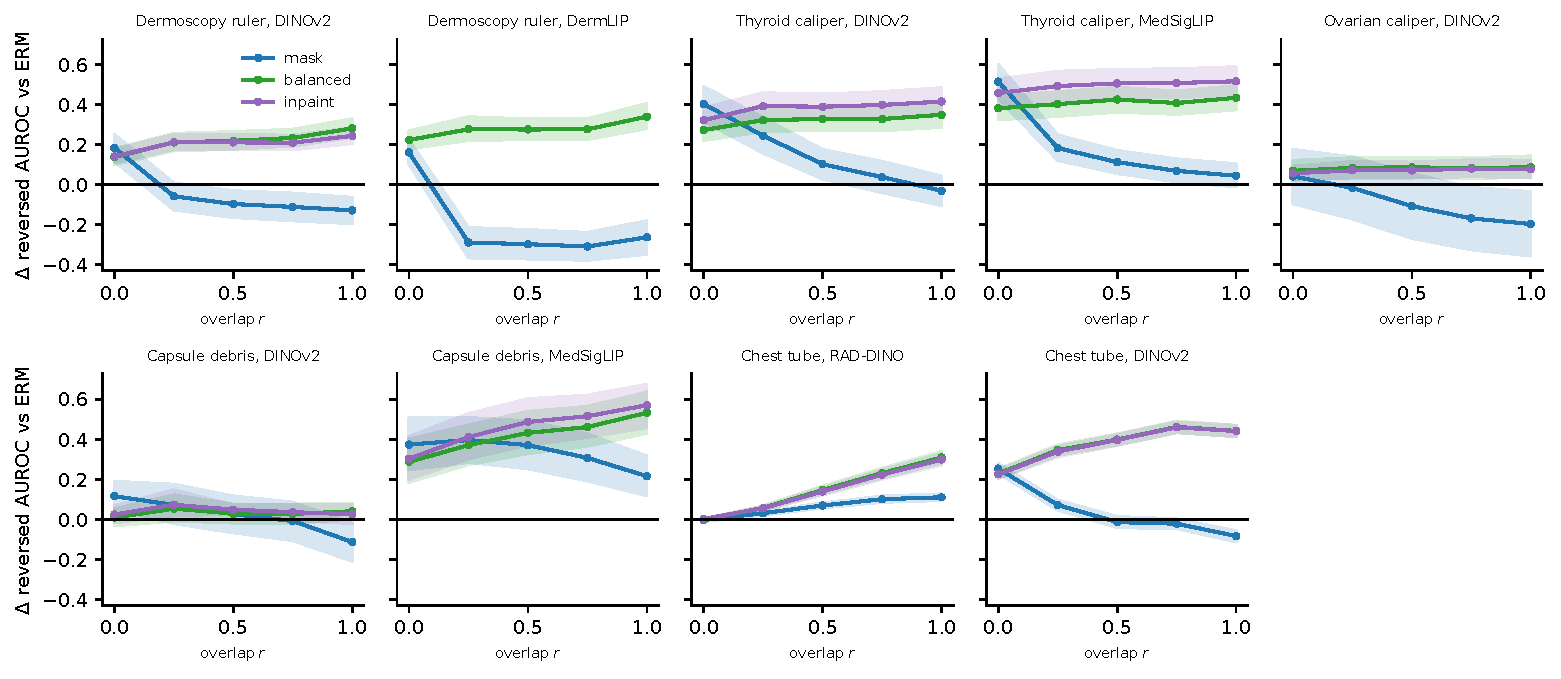
\includegraphics[width=\linewidth]{figures/dose_response_all.pdf}
\caption{Change in reversed-test AUROC versus ERM as a function of overlap, for masking (blue), group balancing (green)
and oracle inpainting (purple), in every controlled sweep (shaded: crossed 95\% CI). Masking falls with overlap in every
panel except the RAD-DINO chest tube.}\label{fig:doseall}\end{figure}
\begin{itemize}[leftmargin=*]\itemsep1pt
\item \textbf{Thyroid calipers.} Masking helps strongly with the caliper outside the nodule (DINOv2
\sTwoThyroidcaliperDINOvTwoZero; MedSigLIP \sTwoThyroidcaliperMedSigLIPZero) and the benefit vanishes at full overlap
(\sTwoThyroidcaliperDINOvTwoFull; \sTwoThyroidcaliperMedSigLIPFull): the law holds as a loss of benefit, not as harm.
Nodules are large relative to the caliper, and the ultrasound background carries little disease information, so
masking costs little besides leaving the caliper.
\item \textbf{Ovarian calipers.} Masking harms at full overlap (\sTwoOvariancaliperDINOvTwoFull) and its benefit outside
the tumour is not significant (\sTwoOvariancaliperDINOvTwoZero): MMOTU tumours fill much of the frame, so little
background is removed, and the test set is small (64 images).
\item \textbf{Capsule debris.} With DINOv2 the sweep reverses (\sTwoCapsuledebrisDINOvTwoZero{} to
\sTwoCapsuledebrisDINOvTwoFull). With MedSigLIP masking still helps at full overlap (\sTwoCapsuledebrisMedSigLIPFull)
but less than outside (\sTwoCapsuledebrisMedSigLIPZero; interaction \sTwoCapsuledebrisMedSigLIPInter): the box ROI
contains much normal mucosa, so masking removes little of the lesion's context.
\item \textbf{Chest tube --- the boundary.} With RAD-DINO the ERM model ignores a tube outside the lungs (reversed
\sTwoCxrErmRevZero{} versus clean \sTwoCxrErmCleanZero{} at no overlap), so masking has nothing to remove at $r=0$; at
full overlap ERM collapses (\sTwoCxrErmRevOneZeroZero) and the masked model less so (\sTwoCxrMaskRevOneZeroZero). The
interaction is negative. With DINOv2, which does use the extra-pulmonary tube (reversed \sTwoCxrDinoErmRevZero{} versus
clean \sTwoCxrDinoErmCleanZero), the law holds (\sTwoChesttubeDINOvTwoInter). The law's premise is that the encoder
uses the out-of-ROI artifact; when it does not, masking cannot help outside and the law does not apply.
\item \textbf{The artifact-targeting arms} (inpainting, balancing, DFR, paired LEACE) help at both overlaps in every
modality except where the intervals are wide (ovary, DINOv2 capsule; Table~\ref{tab:otherarms}). None of them shows the
positive location interaction of masking; most show a small negative one, because ERM relies more on an artifact that
sits on the lesion and there is more for them to remove.
\end{itemize}
{\scriptsize
\begin{longtable}{p{2.6cm}p{3.2cm}ccc}
\caption{All baseline arms in the controlled sweeps of the other modalities: ERM's clean and reversed AUROC and each arm's change in reversed-test AUROC versus ERM at no and at full overlap (crossed CIs). The last column is the arm's own location interaction ($[\cdot]_{r=0}-[\cdot]_{r=1}$); an arm that does not depend on where the artifact sits has an interaction near zero.}\label{tab:otherarms}\\\toprule
Sweep & Arm & $r=0$ & $r=1$ & Location interaction \\\midrule
\endfirsthead
\toprule Sweep & Arm & $r=0$ & $r=1$ & Location interaction \\\midrule
\endhead
\bottomrule
\endlastfoot
Thyroid caliper, DINOv2 & ERM (AUROC: clean; reversed) & 0.666; 0.417 & 0.643; 0.325 & --- \\
 & masking $-$ ERM & $+0.402$ [$+0.315, +0.489$] & $-0.030$ [$-0.105, +0.042$] & $+0.433$ [$+0.362, +0.507$] \\
 & oracle inpainting $-$ ERM & $+0.321$ [$+0.261, +0.383$] & $+0.415$ [$+0.348, +0.484$] & $-0.093$ [$-0.124, -0.065$] \\
 & group-balanced $-$ ERM & $+0.273$ [$+0.220, +0.328$] & $+0.349$ [$+0.286, +0.415$] & $-0.076$ [$-0.106, -0.048$] \\
 & DFR $-$ ERM & $+0.299$ [$+0.228, +0.374$] & $+0.384$ [$+0.298, +0.472$] & $-0.085$ [$-0.123, -0.050$] \\
 & paired LEACE $-$ ERM & $+0.324$ [$+0.264, +0.386$] & $+0.420$ [$+0.353, +0.488$] & $-0.096$ [$-0.129, -0.066$] \\
Thyroid caliper, MedSigLIP & ERM (AUROC: clean; reversed) & 0.742; 0.320 & 0.723; 0.260 & --- \\
 & masking $-$ ERM & $+0.514$ [$+0.430, +0.600$] & $+0.044$ [$-0.011, +0.104$] & $+0.470$ [$+0.388, +0.556$] \\
 & oracle inpainting $-$ ERM & $+0.457$ [$+0.388, +0.527$] & $+0.516$ [$+0.442, +0.589$] & $-0.059$ [$-0.089, -0.031$] \\
 & group-balanced $-$ ERM & $+0.381$ [$+0.324, +0.442$] & $+0.433$ [$+0.373, +0.494$] & $-0.052$ [$-0.084, -0.020$] \\
 & DFR $-$ ERM & $+0.437$ [$+0.370, +0.505$] & $+0.484$ [$+0.409, +0.561$] & $-0.047$ [$-0.086, -0.008$] \\
 & paired LEACE $-$ ERM & $+0.460$ [$+0.389, +0.531$] & $+0.517$ [$+0.442, +0.587$] & $-0.057$ [$-0.089, -0.027$] \\
Ovarian caliper, DINOv2 & ERM (AUROC: clean; reversed) & 0.668; 0.656 & 0.677; 0.635 & --- \\
 & masking $-$ ERM & $+0.041$ [$-0.096, +0.175$] & $-0.197$ [$-0.357, -0.035$] & $+0.238$ [$+0.144, +0.340$] \\
 & oracle inpainting $-$ ERM & $+0.057$ [$+0.025, +0.092$] & $+0.077$ [$+0.034, +0.122$] & $-0.021$ [$-0.047, +0.004$] \\
 & group-balanced $-$ ERM & $+0.069$ [$+0.020, +0.121$] & $+0.087$ [$+0.034, +0.143$] & $-0.018$ [$-0.048, +0.009$] \\
 & DFR $-$ ERM & $+0.013$ [$-0.079, +0.102$] & $+0.047$ [$-0.049, +0.142$] & $-0.034$ [$-0.077, +0.005$] \\
 & paired LEACE $-$ ERM & $+0.056$ [$+0.023, +0.093$] & $+0.073$ [$+0.031, +0.119$] & $-0.017$ [$-0.044, +0.011$] \\
Capsule debris, DINOv2 & ERM (AUROC: clean; reversed) & 0.853; 0.822 & 0.849; 0.797 & --- \\
 & masking $-$ ERM & $+0.116$ [$+0.052, +0.191$] & $-0.112$ [$-0.209, -0.019$] & $+0.228$ [$+0.144, +0.324$] \\
 & oracle inpainting $-$ ERM & $+0.024$ [$-0.016, +0.069$] & $+0.026$ [$-0.020, +0.074$] & $-0.002$ [$-0.026, +0.024$] \\
 & group-balanced $-$ ERM & $+0.009$ [$-0.032, +0.053$] & $+0.041$ [$+0.004, +0.081$] & $-0.032$ [$-0.073, +0.001$] \\
 & DFR $-$ ERM & $+0.030$ [$-0.034, +0.090$] & $+0.049$ [$-0.016, +0.114$] & $-0.019$ [$-0.041, +0.001$] \\
 & paired LEACE $-$ ERM & $+0.035$ [$+0.014, +0.061$] & $+0.059$ [$+0.030, +0.094$] & $-0.023$ [$-0.043, -0.006$] \\
Capsule debris, MedSigLIP & ERM (AUROC: clean; reversed) & 0.902; 0.586 & 0.887; 0.302 & --- \\
 & masking $-$ ERM & $+0.374$ [$+0.248, +0.509$] & $+0.216$ [$+0.118, +0.317$] & $+0.158$ [$+0.012, +0.314$] \\
 & oracle inpainting $-$ ERM & $+0.303$ [$+0.201, +0.414$] & $+0.570$ [$+0.459, +0.675$] & $-0.267$ [$-0.388, -0.145$] \\
 & group-balanced $-$ ERM & $+0.288$ [$+0.185, +0.402$] & $+0.533$ [$+0.430, +0.636$] & $-0.245$ [$-0.359, -0.130$] \\
 & DFR $-$ ERM & $+0.294$ [$+0.186, +0.416$] & $+0.575$ [$+0.453, +0.695$] & $-0.281$ [$-0.398, -0.160$] \\
 & paired LEACE $-$ ERM & $+0.319$ [$+0.212, +0.433$] & $+0.608$ [$+0.499, +0.711$] & $-0.289$ [$-0.405, -0.171$] \\
Chest tube, RAD-DINO & ERM (AUROC: clean; reversed) & 0.915; 0.913 & 0.907; 0.614 & --- \\
 & masking $-$ ERM & $-0.002$ [$-0.010, +0.005$] & $+0.111$ [$+0.095, +0.127$] & $-0.113$ [$-0.129, -0.097$] \\
 & oracle inpainting $-$ ERM & $+0.003$ [$+0.002, +0.004$] & $+0.299$ [$+0.271, +0.329$] & $-0.297$ [$-0.326, -0.267$] \\
 & group-balanced $-$ ERM & $+0.000$ [$-0.004, +0.004$] & $+0.309$ [$+0.280, +0.339$] & $-0.309$ [$-0.338, -0.281$] \\
 & DFR $-$ ERM & $-0.014$ [$-0.022, -0.007$] & $+0.280$ [$+0.248, +0.313$] & $-0.294$ [$-0.328, -0.262$] \\
 & paired LEACE $-$ ERM & $+0.003$ [$+0.002, +0.004$] & $+0.287$ [$+0.259, +0.316$] & $-0.284$ [$-0.314, -0.255$] \\
Chest tube, DINOv2 & ERM (AUROC: clean; reversed) & 0.859; 0.629 & 0.852; 0.410 & --- \\
 & masking $-$ ERM & $+0.254$ [$+0.230, +0.278$] & $-0.083$ [$-0.112, -0.057$] & $+0.337$ [$+0.312, +0.364$] \\
 & oracle inpainting $-$ ERM & $+0.225$ [$+0.204, +0.247$] & $+0.442$ [$+0.413, +0.470$] & $-0.216$ [$-0.235, -0.198$] \\
 & group-balanced $-$ ERM & $+0.229$ [$+0.206, +0.251$] & $+0.442$ [$+0.414, +0.470$] & $-0.214$ [$-0.231, -0.196$] \\
 & DFR $-$ ERM & $+0.218$ [$+0.197, +0.240$] & $+0.433$ [$+0.406, +0.460$] & $-0.214$ [$-0.234, -0.196$] \\
 & paired LEACE $-$ ERM & $+0.233$ [$+0.212, +0.255$] & $+0.452$ [$+0.424, +0.481$] & $-0.219$ [$-0.238, -0.202$] \\
\end{longtable}}


\subsection{Sensitivity to the interval estimator}
As in Stage~1, both estimators were computed on the same predictions of the other-modality sweeps
(Table~\ref{tab:estcheck}): the crossed intervals are wider by a median factor of \sTwoEstMed; \sTwoEstLost{} of
\sTwoEstN{} contrasts lose significance and none gains it (Table~\ref{tab:estchanges}). Every statement in this report
uses the crossed intervals, so these changes are already reflected in the text: in particular, MedSigLIP's small benefit
at full thyroid overlap and the ovarian harm at 50\% overlap are not claimed.
\begin{table}[H]\centering\scriptsize
\caption{The sweeps of the other modalities under the per-seed and the crossed estimator (same predictions; baseline arms only).}\label{tab:estcheck}
\begin{tabular}{p{5.0cm}p{1.4cm}p{2.6cm}p{2.6cm}p{2.4cm}}\toprule
Result group & Intervals & Excluded 0 only with the per-seed estimator & Excluded 0 only with the crossed estimator & Median width ratio (crossed / per-seed) \\\midrule
synthetic/\allowbreak{}capsule & 60 & 9 & 0 & 1.72 \\
synthetic/\allowbreak{}nih\_ptx & 30 & 0 & 0 & 1.44 \\
synthetic/\allowbreak{}ovary & 30 & 1 & 0 & 1.59 \\
synthetic/\allowbreak{}thyroid & 60 & 1 & 0 & 1.37 \\
\textbf{all} & 180 & 11 & 0 & 1.45 \\
\bottomrule\end{tabular}
\end{table}

\begin{table}[H]\centering\scriptsize
\caption{Contrasts of the other-modality sweeps whose verdict depends on the estimator.}\label{tab:estchanges}
\begin{tabular}{p{4.2cm}p{5.2cm}p{3.3cm}p{2.6cm}}\toprule
Result & Contrast & Crossed estimate [95\% CI] & Verdict vs per-seed estimator \\\midrule
synthetic/\allowbreak{}thyroid/\allowbreak{}medsiglip448\_caliper\_corr\_main & 1.0 /\allowbreak{} mask /\allowbreak{} erm /\allowbreak{} test\_rev & $+0.044$ [$-0.011, +0.104$] & no longer excludes 0 \\
synthetic/\allowbreak{}capsule/\allowbreak{}dino518\_debris\_corr\_main & 0.0 /\allowbreak{} inpaint /\allowbreak{} erm /\allowbreak{} test\_rev & $+0.024$ [$-0.016, +0.069$] & no longer excludes 0 \\
synthetic/\allowbreak{}capsule/\allowbreak{}dino518\_debris\_corr\_main & 0.75 /\allowbreak{} inpaint /\allowbreak{} erm /\allowbreak{} test\_rev & $+0.036$ [$-0.005, +0.074$] & no longer excludes 0 \\
synthetic/\allowbreak{}capsule/\allowbreak{}dino518\_debris\_corr\_main & 1.0 /\allowbreak{} inpaint /\allowbreak{} erm /\allowbreak{} test\_rev & $+0.026$ [$-0.020, +0.074$] & no longer excludes 0 \\
synthetic/\allowbreak{}capsule/\allowbreak{}dino518\_debris\_corr\_main & 0.5 /\allowbreak{} balanced /\allowbreak{} erm /\allowbreak{} test\_rev & $+0.030$ [$-0.018, +0.076$] & no longer excludes 0 \\
synthetic/\allowbreak{}capsule/\allowbreak{}dino518\_debris\_corr\_main & 0.75 /\allowbreak{} balanced /\allowbreak{} erm /\allowbreak{} test\_rev & $+0.028$ [$-0.023, +0.076$] & no longer excludes 0 \\
synthetic/\allowbreak{}capsule/\allowbreak{}dino518\_debris\_corr\_main & 0.0 /\allowbreak{} dfr /\allowbreak{} erm /\allowbreak{} test\_rev & $+0.030$ [$-0.034, +0.090$] & no longer excludes 0 \\
synthetic/\allowbreak{}capsule/\allowbreak{}dino518\_debris\_corr\_main & 0.5 /\allowbreak{} dfr /\allowbreak{} erm /\allowbreak{} test\_rev & $+0.048$ [$-0.014, +0.110$] & no longer excludes 0 \\
synthetic/\allowbreak{}capsule/\allowbreak{}dino518\_debris\_corr\_main & 0.75 /\allowbreak{} dfr /\allowbreak{} erm /\allowbreak{} test\_rev & $+0.055$ [$-0.010, +0.122$] & no longer excludes 0 \\
synthetic/\allowbreak{}capsule/\allowbreak{}dino518\_debris\_corr\_main & 1.0 /\allowbreak{} dfr /\allowbreak{} erm /\allowbreak{} test\_rev & $+0.049$ [$-0.016, +0.114$] & no longer excludes 0 \\
synthetic/\allowbreak{}ovary/\allowbreak{}dino518\_caliper\_corr\_main & 0.5 /\allowbreak{} mask /\allowbreak{} erm /\allowbreak{} test\_rev & $-0.107$ [$-0.269, +0.054$] & no longer excludes 0 \\
\bottomrule\end{tabular}
\end{table}


\section{What failed or changed}\label{sec:changed}
\begin{itemize}[leftmargin=*]\itemsep1pt
\item \textbf{Harm at full overlap is not universal.} The robust statement is the \emph{interaction} (\sTwoNInterPos{}
of \sTwoNSweeps); harm at full overlap is significant in \sTwoNHarmFull{} of \sTwoNSweeps{} sweeps.
\item \textbf{Two lesion-size cells are not significant} (large lesions at full overlap, medium lesions at 50\%): harm
is ordered by lesion size, not monotone in every cell.
\item \textbf{Chest radiography with RAD-DINO contradicts the law}, as a failure of its premise. It was registered as a
confirmation and is reported as a boundary case.
\item \textbf{The counterfactual mechanism holds in \sTwoCfNPos{} of \sTwoCfN{} sweeps}: not for thyroid calipers (equal
sensitivity) and reversed for the chest tube with RAD-DINO.
\item \textbf{The ovarian sweep has no significant benefit outside the ROI}, so its interaction rests on the harm side.
\item \textbf{Reproducibility of the capsule split.} The capsule sweep's split is produced by a seeded shuffle of the
group list; rebuilding the cohort (a re-derived contamination mask moved a few frames across the 5\% threshold) re-dealt
the split, and only 32 of 71 artifact-bearing test frames of an earlier build recur. Point estimates of that sweep moved
by up to about 0.2, while the location interaction kept its sign and significance. The split is now frozen with the
cohort file.
\end{itemize}

\section{Anticipated questions}
\paragraph{Why not simply show saliency maps?} They show where a model looks, not how much its decision depends on the
artifact, and they are unstable for frozen encoders with linear heads. The same-head counterfactual answers the causal
question directly on the same image.
\paragraph{If masking removes context, why is the occlusion control not harmed?} Because in the occlusion control the
ruler is uninformative: the head does not need it, so keeping it costs nothing, and the context lost by masking is
small for this task. The harm in the sweep appears only when the retained ruler predicts the label in training.
\paragraph{Why does dilation make things worse at 50\% overlap?} Because it makes more of the ruler visible (retention
0.50 $\to$ 0.95) while adding only a thin rim of context. The shortcut becomes stronger; the head uses it more.
\paragraph{Why does the harm not grow at 100\% overlap when the mask is dilated?} The ruler is already fully visible;
dilation only adds skin. If harm were about the ruler's share of the image it would fall; it does not.
\paragraph{Why do the artifact-targeting arms help \emph{more} when the artifact is inside?} ERM relies more on a ruler
on the lesion (its reversed AUROC is lower at $r=1$), so removing that reliance gains more. Their gain does not depend
on the ROI.
\paragraph{Why does thyroid show loss of benefit rather than harm?} The ultrasound background contains little disease
information, so masking loses almost nothing besides failing to remove the caliper; ERM is already caliper-driven, and
masking leaves it so. Harm needs masking to remove disease evidence as well.
\paragraph{Why is the chest tube a boundary and not a failure?} The law compares what masking removes outside and
inside the ROI. RAD-DINO does not use the out-of-lung tube at all (reversed $\approx$ clean AUROC), so there is nothing to
remove outside and the comparison has no content. DINOv2 uses the tube and shows the law.
\paragraph{Are 3 seeds enough?} For the interactions, yes: the intervals include the variation of the fixed test set,
and \sTwoNInterPos{} of \sTwoNSweeps{} exclude zero. Individual cells in small cohorts (ovary) are imprecise and are
interpreted only through the interaction.
\paragraph{Could the synthetic artifacts be unrealistic?} Yes, and that is their purpose: they isolate location.
Whether the law holds for artifacts that clinicians actually produce is a separate question that synthetic sweeps
cannot answer.

\section{Conclusion}
\textbf{Supported.} The location law in its interaction form (Q2a) holds in \sTwoNInterPos{} of \sTwoNSweeps{}
controlled sweeps across five modalities and four encoders. The mechanism (Q2b) is retention with amplified reliance:
occlusion alone does not harm, harm follows the visibility of the artifact under dilation, and the masked head's
same-image reliance on an in-ROI artifact is about \sTwoDpRatioFull{} times that of ERM for the ruler (\sTwoDpDiffFull)
and significantly higher in \sTwoCfNPos{} of \sTwoCfN{} sweeps. \textbf{Qualified.} Harm at full overlap is
setting-dependent; the lesion-size gradient is an ordering. \textbf{Not supported.} The law for an encoder that ignores
the out-of-ROI artifact (chest tube, RAD-DINO). The practical reading is: masking removes what lies outside the ROI and
concentrates the model on what lies inside; whether that helps depends on where the shortcut sits.

\section{Questions for the supervisor}
\begin{enumerate}\itemsep1pt
\item Should the thesis state the law in its interaction form only (robust) and treat harm at full overlap as
setting-dependent, or keep harm as the headline for dermoscopy, where it holds with every encoder?
\item The counterfactual mechanism holds in \sTwoCfNPos{} of \sTwoCfN{} sweeps. Is the thyroid result (the unmasked model
is already as reliant on an in-nodule caliper as the masked one) best presented as a limitation or as a second route to
the same outcome?
\item Is it acceptable to present chest radiography with RAD-DINO as a boundary of the law rather than as a failed
confirmation, given that it was registered as a confirmation?
\end{enumerate}

\bibliographystyle{plainnat}
\bibliography{../common/references}
\end{document}
